%%%%%%%%%%%%%%%%%%%%%%%%%%%%%%%%%%%%%%%%%%%%%%%%%%%%%%%%%%%%%%%%%%%%%%%%%%%%%%%%
% CSC2059 Practical 7
%%%%%%%%%%%%%%%%%%%%%%%%%%%%%%%%%%%%%%%%%%%%%%%%%%%%%%%%%%%%%%%%%%%%%%%%%%%%%%%%

\documentclass{csc2059practical}

% Additional packages used by this practical.
% TikZ figures will be added during the visual design pass.
\usepackage{tikz}
\usetikzlibrary{arrows.meta, positioning, fit, backgrounds}
\usepackage{fontawesome5}
\usepackage{booktabs}

\setpracticalnumber{7}

\setpracticaltitle{Engineering Recursive Algorithms for Tree Structures}

\setpracticalsubtitle{From Smaller Problems to Reusable Tree Algorithms}

\setpracticalauthor{
Dr Giuseppe Trombino\\
School of Electronics, Electrical Engineering and Computer Science\\
Queen's University Belfast
}
\setpracticaldate{}

\usetikzlibrary{arrows.meta, positioning, backgrounds, calc}
\usepackage{forest}
\usepackage{fontawesome5}

\begin{document}

\maketitle

\tableofcontents
\clearpage

%%%%%%%%%%%%%%%%%%%%%%%%%%%%%%%%%%%%%%%%%%%%%%%%%%%%%%%%%%%%%%%%%%%%%%%%%%%%%%%%
% Introduction
%%%%%%%%%%%%%%%%%%%%%%%%%%%%%%%%%%%%%%%%%%%%%%%%%%%%%%%%%%%%%%%%%%%%%%%%%%%%%%%%

\frontsection{Introduction}

Recursion is often introduced through short mathematical examples such as
factorial. These examples can make the syntax appear simple while hiding the
more difficult question:

\begin{quote}
How do we recognise that a problem can be solved recursively?
\end{quote}

Writing a recursive function is rarely the hardest part. The real challenge is
identifying:

\begin{enumerate}
    \item the smallest version of the problem that already has an answer;
    \item a smaller version of the current problem;
    \item the work that remains after the smaller problem has been solved.
\end{enumerate}

In this practical, you will use these three questions as a repeatable design
process. You will first apply them to a small numerical problem, then recognise
the same reasoning in a familiar folder hierarchy, and finally use it to
construct, navigate and search binary trees.

The practical deliberately begins with the problem rather than the code. You
will predict and trace recursive behaviour before implementing it. Public
Catch2 tests will then guide you through increasingly capable solutions using
the same engineering rhythm used throughout CSC2059:

\begin{quote}
Predict $\rightarrow$ Observe $\rightarrow$ Understand $\rightarrow$ Test
$\rightarrow$ Implement $\rightarrow$ Refine
\end{quote}

By the end, the examples will have changed, but the recursive reasoning will
remain recognisable.

\begin{engineeringquestion}
How can we design an algorithm when a problem is made from smaller versions of
itself?
\end{engineeringquestion}

\begin{importantnote}
This practical is not about replacing loops with recursion.

The aim is to recognise problems for which recursive decomposition provides a
natural and reusable solution.
\end{importantnote}

%%%%%%%%%%%%%%%%%%%%%%%%%%%%%%%%%%%%%%%%%%%%%%%%%%%%%%%%%%%%%%%%%%%%%%%%%%%%%%%%
% Learning Outcomes
%%%%%%%%%%%%%%%%%%%%%%%%%%%%%%%%%%%%%%%%%%%%%%%%%%%%%%%%%%%%%%%%%%%%%%%%%%%%%%%%

\begin{learningoutcomes}

By the end of this practical, you should be able to:

\begin{itemize}
    \item explain how a recursive problem is divided into a base case, smaller
          subproblems and remaining work;
    \item trace recursive calls and the values returned as execution unwinds;
    \item implement a recursive function using an appropriate stopping
          condition;
    \item construct and navigate a dynamically allocated binary tree;
    \item use public tests to develop a recursive tree-search algorithm
          incrementally;
    \item calculate the depth of balanced, skewed and uneven binary trees;
    \item generalise a concrete recursive algorithm using a C++ function
          template;
    \item recognise how the same recursive reasoning applies beyond one
          particular data structure.
\end{itemize}

\end{learningoutcomes}

%%%%%%%%%%%%%%%%%%%%%%%%%%%%%%%%%%%%%%%%%%%%%%%%%%%%%%%%%%%%%%%%%%%%%%%%%%%%%%%%
% Estimated Effort
%%%%%%%%%%%%%%%%%%%%%%%%%%%%%%%%%%%%%%%%%%%%%%%%%%%%%%%%%%%%%%%%%%%%%%%%%%%%%%%%

\begin{infobox}[Estimated Effort]

This practical has been designed for a two-hour session.

The approximate distribution of effort is:

\begin{center}
\begin{tabular}{ll}
\toprule
\textbf{Activity} & \textbf{Suggested Time} \\
\midrule
Part A --- Discovering Recursive Thinking & 20--25 minutes \\
Part B --- Recognising Recursive Structures & 5--10 minutes \\
Part C --- Constructing and Searching a Binary Tree & 35--45 minutes \\
Part D --- Reusing and Generalising the Pattern & 25--35 minutes \\
Part E --- Returning to the Original Problem & 5--10 minutes \\
\bottomrule
\end{tabular}
\end{center}
\end{infobox}

The timings are a guide rather than a deadline. Work through the demonstrations
and tests in order. If you become stuck, seek help early rather than skipping
ahead, because each part develops the reasoning required by the next.


%%%%%%%%%%%%%%%%%%%%%%%%%%%%%%%%%%%%%%%%%%%%%%%%%%%%%%%%%%%%%%%%%%%%%%%%%%%%%%%%
% Before You Begin
%%%%%%%%%%%%%%%%%%%%%%%%%%%%%%%%%%%%%%%%%%%%%%%%%%%%%%%%%%%%%%%%%%%%%%%%%%%%%%%%

\frontsection{Before You Begin}

This practical is designed to work as a learning unit in its own right.
However, it builds on several ideas you have already used elsewhere in the
module.

Before beginning, check that you can recognise the following:

\begin{itemize}
    \item compiling and running C++ programs using Visual Studio Code and a
          Makefile;
    \item running public Catch2 tests and interpreting a failed assertion;
    \item separating public declarations in header files from implementations
          in source files;
    \item using pointers and \mintinline{cpp}{nullptr};
    \item allocating an object with \mintinline{cpp}{new} and releasing it with
          \mintinline{cpp}{delete};
    \item following member pointers using the
          \mintinline{cpp}{->} operator;
    \item reading a simple C++ class template;
    \item using a failing test to identify the next small behaviour to
          implement.
\end{itemize}

You do not need to be fully confident with recursion before starting. Developing
that confidence is one of the main purposes of the practical.

\begin{importantnote}
The supplied \mintinline{cpp}{TreeNode<T>} owns its left and right subtrees.
Deleting the root therefore deletes the entire tree recursively.

For this ownership model to work correctly, child nodes attached to the tree
must be created dynamically using \mintinline{cpp}{new}. A later section will
explain this in more detail.
\end{importantnote}

\begin{tipbox}
If pointers or dynamic allocation feel unfamiliar, briefly revisit the relevant
material from Practical 3 before beginning Part C. Do not postpone the whole
practical: Parts A and B can still be completed while you refresh those ideas.
\end{tipbox}

%%%%%%%%%%%%%%%%%%%%%%%%%%%%%%%%%%%%%%%%%%%%%%%%%%%%%%%%%%%%%%%%%%%%%%%%%%%%%%%%
% Repository Access
%%%%%%%%%%%%%%%%%%%%%%%%%%%%%%%%%%%%%%%%%%%%%%%%%%%%%%%%%%%%%%%%%%%%%%%%%%%%%%%%

\frontsection{Repository Access}

Access the Practical 7 repository through the link provided on Canvas, then
clone it to your local machine.

Open the cloned folder in Visual Studio Code. Do not create a separate project
or copy individual files elsewhere. The supplied Makefile expects the repository
structure to remain unchanged.

From the repository root, build the starter project:

\begin{terminal}
make
\end{terminal}

A successful build creates executable files inside the \mintinline{text}{bin/}
directory.

Next, run the core public test suite:

\begin{terminal}
make test
\end{terminal}

The repository is supplied in a deliberate starter state. Some tests will pass
and others will fail because several functions still contain TODO markers.
Compilation should succeed, however.

\begin{importantnote}
The test file \mintinline{text}{test05_generic_tree_search.cpp} is not included
in the normal \mintinline{text}{make test} target at the beginning of the
practical.

It introduces a requirement that the initial string-only search function cannot
yet compile against. You will activate it later using a dedicated Makefile
target as part of a guided refactoring exercise.
\end{importantnote}

The two demonstrations can be run using:

\begin{terminal}
make run-example01
make run-example02
\end{terminal}

Run each demonstration only when directed by the guide. They are designed to be
used alongside the surrounding explanation rather than watched in advance.

Throughout the practical:

\begin{itemize}
    \item work on one failing behaviour at a time;
    \item rerun the relevant tests after each change;
    \item keep previously passing tests green;
    \item commit and push regularly using meaningful messages.
\end{itemize}

Suggested commit points include:

\begin{terminal}
git add .
git commit -m "Complete recursive digital root"
git push
\end{terminal}

and later:

\begin{terminal}
git add .
git commit -m "Implement recursive tree search"
git push
\end{terminal}

%%%%%%%%%%%%%%%%%%%%%%%%%%%%%%%%%%%%%%%%%%%%%%%%%%%%%%%%%%%%%%%%%%%%%%%%%%%%%%%%
% Repository Tour
%%%%%%%%%%%%%%%%%%%%%%%%%%%%%%%%%%%%%%%%%%%%%%%%%%%%%%%%%%%%%%%%%%%%%%%%%%%%%%%%

\frontsection{Repository Tour}

The repository is organised around the order in which demonstrations and tests
should be used. Example and test numbers indicate execution order; they do not
necessarily match the lettering of the guide sections.

\begin{center}
\begin{tabular}{ll}
\toprule
\textbf{Path} & \textbf{Purpose} \\
\midrule
\texttt{examples/} & Complete demonstrations used to observe new ideas. \\
\texttt{include/} & Public interfaces and template implementations. \\
\texttt{src/} & Non-template starter implementations and construction code. \\
\texttt{tests/} & Public Catch2 tests that guide each implementation step. \\
\texttt{external/} & The supplied Catch2 testing framework. \\
\texttt{bin/} & Generated executables created by the Makefile. \\
\texttt{Makefile} & Builds and runs demonstrations and tests. \\
\texttt{README.md} & A concise repository survival guide. \\
\bottomrule
\end{tabular}
\end{center}

The main files are shown below.

\subsection*{\texttt{examples/}}

\noindent
\texttt{example01\_recursive\_thinking.cpp}

\smallskip

A guided demonstration of recursive calls, waiting work and returned values
using the reciprocal-square sum.

\medskip

\noindent
\texttt{example02\_binary\_tree\_introduction.cpp}

\smallskip

Supports manual pointer navigation through the completed binary tree and
introduces the limitation of hard-coded paths.

\bigskip


\subsection*{\texttt{include/} and \texttt{src/}}

\noindent
\texttt{recursion\_exercises.h},
\texttt{recursion\_exercises.cpp}, and
\texttt{test01\_recursive\_thinking.cpp}

\smallskip

These files contain the Digital Root interface, starter implementation and
public tests used in Part A. The source file also contains the supplied
\mintinline{cpp}{digitSum()} helper.

\medskip

\noindent
\texttt{TreeNode.h}

\smallskip

Defines the generic binary-tree node, its left and right child pointers, and
its recursive destructor.

\medskip

\noindent
\texttt{tree\_exercises.h} and
\texttt{tree\_exercises.cpp}

\smallskip

Declare and implement the function used to construct the shared simplified
file tree.

\medskip

\noindent
\texttt{tree\_algorithms.h} and
\texttt{tree\_algorithms.cpp}

\smallskip

Contain the recursive tree algorithms developed later in the practical. The
initial search function is string-specific, while the template starter for
\mintinline{cpp}{depth()} must remain visible in the header.

\bigskip


\subsection*{\texttt{tests/}}

\noindent
\texttt{test01\_recursive\_thinking.cpp}

\smallskip

Guides the Digital Root implementation from single-digit base cases to values
requiring repeated reduction.

\medskip

\noindent
\texttt{test02\_binary\_tree\_construction.cpp}

\smallskip

Reveals the required binary-tree structure one level at a time and verifies
that the lowest-level folders are leaves.

\medskip

\noindent
\texttt{test03\_recursive\_tree\_search.cpp}

\smallskip

Guides recursive search through an empty tree, the current node, the left
subtree, the right subtree and missing values.

\medskip

\noindent
\texttt{test04\_tree\_depth.cpp}

\smallskip

Checks the depth of empty, single-node, balanced, skewed and uneven trees.

\medskip

\noindent
\texttt{test05\_generic\_tree\_search.cpp}

\smallskip

Introduces integer trees and exposes the limitation of the initial
string-specific search interface. This test is activated later using its
dedicated Makefile target.

\medskip

\noindent
\texttt{test\_main.cpp}

\smallskip

Provides the Catch2 entry point shared by the numbered public test files.

The practical follows this engineering journey:

\begin{center}
\begin{tabular}{p{0.12\textwidth} p{0.76\textwidth}}
\toprule
\textbf{Part} & \textbf{Engineering Journey} \\
\midrule
A & Learn how to identify and trace a recursive solution. \\
B & Recognise the same reasoning in a familiar folder-search problem. \\
C & Simplify the hierarchy, construct a binary tree and automate its search. \\
D & Reuse the recursive pattern to measure trees and generalise the algorithm. \\
E & Return to the original hierarchy and identify what truly depended on the
    binary-tree simplification. \\
\bottomrule
\end{tabular}
\end{center}

\begin{reflectionbox}
Before moving into Part A, look over the repository one more time.

Which files are complete demonstrations?

Which files contain TODO markers?

Which test introduces a requirement that is deliberately unavailable at the
start?

Understanding the role of each file will make it easier to follow the practical
without jumping ahead.
\end{reflectionbox}

%%%%%%%%%%%%%%%%%%%%%%%%%%%%%%%%%%%%%%%%%%%%%%%%%%%%%%%%%%%%%%%%%%%%%%%%%%%%%%%%
% Practical 7 -- Part A
%%%%%%%%%%%%%%%%%%%%%%%%%%%%%%%%%%%%%%%%%%%%%%%%%%%%%%%%%%%%%%%%%%%%%%%%%%%%%%%%
\clearpage

\section{Part A -- Discovering Recursive Thinking}

\begin{learningoutcomes}
By the end of this part, you should be able to:

\begin{itemize}
    \item identify the base case in a recursive problem;
    \item describe how a problem is reduced to a smaller version of itself;
    \item explain what work waits while a recursive call is completed;
    \item trace both the downward sequence of recursive calls and the upward
          sequence of returned values;
    \item implement a small recursive function using public tests.
\end{itemize}
\end{learningoutcomes}

\begin{infobox}[Estimated Effort]
Estimated time: \textbf{20--25 minutes}
\end{infobox}

Recursion is often presented as a compact piece of C++ syntax. That can make the
finished function look deceptively simple while leaving the difficult reasoning
unexplained.

In this part, you will not begin by converting a loop into recursion. Instead,
you will begin with the problem itself and use three questions to design the
solution before seeing the code.

\begin{importantnote}
Do not skip directly to the demonstration source file.

The purpose of the next activity is to practise recognising a recursive
solution before the implementation is revealed.
\end{importantnote}

\subsection{The Three Questions}

When considering a recursive solution, ask:

\begin{enumerate}
    \item \textbf{What is the smallest problem that already has an answer?}
    \item \textbf{How can the current problem be reduced to a smaller version
          of itself?}
    \item \textbf{If the smaller problem is solved, what work remains to solve
          the current problem?}
\end{enumerate}

These questions correspond to the main parts of a recursive algorithm:

\begin{center}
\begin{tabular}{p{0.39\textwidth} p{0.39\textwidth}}
\toprule
\textbf{Design Question} & \textbf{Recursive Role} \\
\midrule
What is the smallest problem? & The base case stops the recursion. \\
How does the problem become smaller? & The recursive call moves towards
the base case. \\
What work remains? & The current call uses the returned result to complete its
own answer. \\
\bottomrule
\end{tabular}
\end{center}

The first two questions explain how recursion moves \emph{downwards}. The third
explains what happens when the calls begin returning \emph{upwards}.

That return journey is easy to overlook. A recursive call does not erase the
current problem. The current call pauses, remembers its local information, and
waits for the smaller problem to return.

\begin{figure}[htbp]
    \centering

    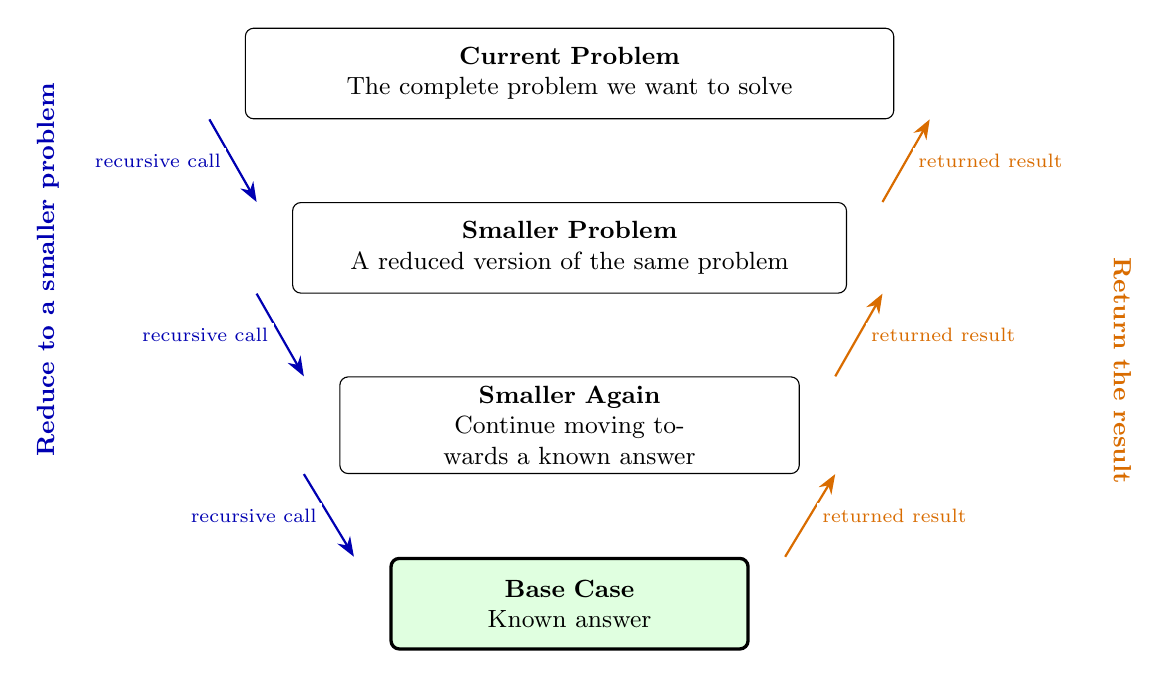
\begin{tikzpicture}[
        problem/.style={
            draw,
            rounded corners=3pt,
            minimum height=1.15cm,
            align=center,
            font=\small
        },
        basecase/.style={
            problem,
            fill=green!12,
            very thick
        },
        callarrow/.style={
            -{Stealth[length=2.5mm]},
            thick,
            blue!70!black
        },
        returnarrow/.style={
            -{Stealth[length=2.5mm]},
            thick,
            orange!85!black
        },
        arrowlabel/.style={
            font=\scriptsize,
            fill=white,
            inner sep=2pt
        },
        node distance=1.05cm
    ]

        % ---------------------------------------------------------------------
        % Progressively smaller problems
        % ---------------------------------------------------------------------

        \node[
            problem,
            text width=8.0cm
        ] (problem1) {
            \textbf{Current Problem}\\
            The complete problem we want to solve
        };

        \node[
            problem,
            text width=6.8cm,
            below=of problem1
        ] (problem2) {
            \textbf{Smaller Problem}\\
            A reduced version of the same problem
        };

        \node[
            problem,
            text width=5.6cm,
            below=of problem2
        ] (problem3) {
            \textbf{Smaller Again}\\
            Continue moving towards a known answer
        };

        \node[
            basecase,
            text width=4.3cm,
            below=of problem3
        ] (base) {
            \textbf{Base Case}\\
            Known answer
        };

        % ---------------------------------------------------------------------
        % Downward recursive calls
        % ---------------------------------------------------------------------

        \draw[callarrow]
            ($(problem1.south west)+(-0.45,0)$)
            --
            node[arrowlabel, left=2pt] {recursive call}
            ($(problem2.north west)+(-0.45,0)$);

        \draw[callarrow]
            ($(problem2.south west)+(-0.45,0)$)
            --
            node[arrowlabel, left=2pt] {recursive call}
            ($(problem3.north west)+(-0.45,0)$);

        \draw[callarrow]
            ($(problem3.south west)+(-0.45,0)$)
            --
            node[arrowlabel, left=2pt] {recursive call}
            ($(base.north west)+(-0.45,0)$);

        % ---------------------------------------------------------------------
        % Upward returned results
        % ---------------------------------------------------------------------

        \draw[returnarrow]
            ($(base.north east)+(0.45,0)$)
            --
            node[arrowlabel, right=2pt] {returned result}
            ($(problem3.south east)+(0.45,0)$);

        \draw[returnarrow]
            ($(problem3.north east)+(0.45,0)$)
            --
            node[arrowlabel, right=2pt] {returned result}
            ($(problem2.south east)+(0.45,0)$);

        \draw[returnarrow]
            ($(problem2.north east)+(0.45,0)$)
            --
            node[arrowlabel, right=2pt] {returned result}
            ($(problem1.south east)+(0.45,0)$);

        % ---------------------------------------------------------------------
        % Journey labels
        % ---------------------------------------------------------------------

        \node[
            font=\small\bfseries,
            blue!70!black,
            rotate=90,
            left=2.5cm of problem1
        ] {
            Reduce to a smaller problem
        };

        \node[
            font=\small\bfseries,
            orange!85!black,
            rotate=270,
            right=3.5cm of problem2
        ] {
            Return the result
        };

    \end{tikzpicture}

    \caption{Recursive decomposition: calls reduce the problem until a known
    base case is reached, then returned results travel back through the waiting
    calls.}
    \label{fig:recursive-decomposition}
\end{figure}

\begin{reflectionbox}
Before continuing, explain the following distinction in your own words:

\begin{itemize}
    \item What causes recursive calls to continue moving downwards?
    \item What allows the final result to move back upwards?
\end{itemize}

You do not need formal terminology. Focus on what the program must remember and
what each call must eventually return.
\end{reflectionbox}

\subsection{A Problem That Contains a Smaller Version of Itself}

Consider the sum of the first \(n\) reciprocal square values:

\[
S(n)
=
\frac{1}{1^2}
+
\frac{1}{2^2}
+
\cdots
+
\frac{1}{n^2}
\]

For example:

\[
S(4)
=
\frac{1}{1^2}
+
\frac{1}{2^2}
+
\frac{1}{3^2}
+
\frac{1}{4^2}
\]

Do not write code yet.

Instead, imagine that another function has already calculated \(S(3)\).

\begin{engineeringquestion}
If \(S(3)\) is already known, what additional work is required to calculate
\(S(4)\)?
\end{engineeringquestion}

The only missing contribution is:

\[
\frac{1}{4^2}
\]

Therefore:

\[
S(4)
=
S(3)
+
\frac{1}{4^2}
\]

The same relationship applies for any positive \(n\):

\[
S(n)
=
S(n-1)
+
\frac{1}{n^2}
\]

This expression has already revealed the smaller problem:

\[
S(n-1)
\]

The recursive call does not need to understand the whole sum at once. It needs
only to trust that the smaller problem will return the correct result.

\subsection{Identify the Base Case}

The recursive definition above continually reduces \(n\):

\[
S(4) \rightarrow S(3) \rightarrow S(2) \rightarrow S(1) \rightarrow S(0)
\]



A recursive algorithm must eventually reach a problem that requires no further
recursive call.

For this demonstration, define the empty sum as:

\[
S(0)=0
\]

This gives a clean stopping condition. Once the current problem becomes
\(S(0)\), the answer is already known.

The three questions can now be answered completely:

\begin{center}
\begin{tabular}{p{0.34\textwidth} p{0.54\textwidth}}
\toprule
\textbf{Question} & \textbf{Answer for \(S(n)\)} \\
\midrule
What is the smallest problem? & \(S(0)=0\). \\
How does the problem become smaller? & Replace \(S(n)\) with \(S(n-1)\). \\
What work remains? & Add the current contribution
\(\frac{1}{n^2}\). \\
\bottomrule
\end{tabular}
\end{center}

At this point, the recursive algorithm has been designed even though no C++
code has been shown.

\begin{importantnote}
The code should be the final expression of the reasoning, not the starting
point.

When the base case, smaller problem and waiting work are clear, the recursive
implementation is often short because the difficult thinking has already been
completed.
\end{importantnote}

\subsection{Watch the Recursive Algorithm Execute}

The mathematical reasoning is now complete:

\[
S(n)=S(n-1)+\frac{1}{n^2}
\]

The remaining task is to translate that reasoning into code.

Run the demonstration:

\begin{terminal}
make run-example01
\end{terminal}

The program pauses after every important stage of the recursive execution.
Before pressing Enter each time, try to predict what will happen next.

\begin{importantnote}
The demonstration includes helper functions such as:

\begin{cppcode}
showCurrentProblem(n);
showSmallerProblem(n - 1);
showWaitingWork(n);
showReturnedValue(...);
\end{cppcode}

These functions exist only to explain what the recursive algorithm is doing.
They are not part of the recursive solution itself.
\end{importantnote}

When the program finishes executing, open the implementation:

\begin{terminal}
examples/example01_recursive_thinking.cpp
\end{terminal}

Locate:

\begin{cppcode}
double reciprocalSquareSum(int n)
\end{cppcode}

As the demonstration executes, identify the three decisions you designed earlier.

\subsubsection*{Step 1 -- The Base Case}

Eventually the recursive calls reach:

\[
S(0)
\]

The demonstration now stops making further recursive calls.

Locate the corresponding code:

\begin{cppcode}
if (n == 0)
{
    return 0.0;
}
\end{cppcode}

Ask yourself:

\begin{itemize}
    \item Why is no further recursive call needed?
    \item Why is returning immediately important?
\end{itemize}

\subsubsection*{Step 2 -- The Smaller Problem}

Return to the beginning of the function.

Locate the recursive call:

\begin{cppcode}
const double smallerResult =
    reciprocalSquareSum(n - 1);
\end{cppcode}

Each time the demonstration reports a smaller problem, this is the line being
executed.

Notice that the function does not try to solve the entire problem itself.
Instead, it trusts that the smaller problem will return the correct result.

\subsubsection*{Step 3 -- The Waiting Work}

Once the recursive call returns, the current function resumes.

Locate:

\begin{cppcode}
const double contribution =
    1.0 / (static_cast<double>(n) * n);

const double result =
    smallerResult + contribution;
\end{cppcode}

This is the work that each paused recursive call was waiting to complete.

As the demonstration returns from

\[
S(0)
\rightarrow
S(1)
\rightarrow
S(2)
\rightarrow
S(3)
\rightarrow
S(4)
\]

watch how each call performs its own local calculation before returning to the
previous caller.

\begin{reflectionbox}
Compare the mathematical definition

\[
S(n)=S(n-1)+\frac{1}{n^2}
\]

with the implementation.

\begin{itemize}
    \item Which line represents the base case?
    \item Which line represents the smaller problem?
    \item Which line performs the waiting work?
    \item Which line combines the two pieces to produce the final answer?
\end{itemize}

The C++ implementation should now look like a direct translation of the
reasoning you developed before writing any code.
\end{reflectionbox}

\subsection{Apply the Process: Digital Root}

You will now use the same design process independently.

The \textbf{digital root} of a non-negative integer is found by repeatedly
summing its digits until one digit remains.

For example:

\[
1916
\rightarrow
1+9+1+6
=
17
\rightarrow
1+7
=
8
\]

Therefore, the digital root of \(1916\) is \(8\).

The repository already provides a helper function:

\begin{cppcode}
int digitSum(int value);
\end{cppcode}

You do not need to implement this helper. It calculates one sum of the decimal
digits:

\begin{center}
\begin{tabular}{cc}
\toprule
\textbf{Input} & \textbf{\mintinline{cpp}{digitSum()} Result} \\
\midrule
42 & 6 \\
1916 & 17 \\
9999 & 36 \\
\bottomrule
\end{tabular}
\end{center}

Your task is to implement:

\begin{cppcode}
int digitalRoot(int value);
\end{cppcode}

Before opening the implementation, answer the three questions.

\begin{engineeringquestion}
For \mintinline{cpp}{digitalRoot()}:

\begin{enumerate}
    \item What is the smallest input that already has its final answer?
    \item How can \mintinline{cpp}{digitSum()} create a smaller problem?
    \item Once the smaller problem is solved, is any additional work required?
\end{enumerate}
\end{engineeringquestion}

A single-digit number is already its own digital root. Therefore, values from
\(0\) to \(9\) form the base case.

For a larger value, \mintinline{cpp}{digitSum(value)} moves the problem towards
that base case. If its result is still larger than \(9\), the same process must
be applied again.

\begin{figure}[htbp]
    \centering

    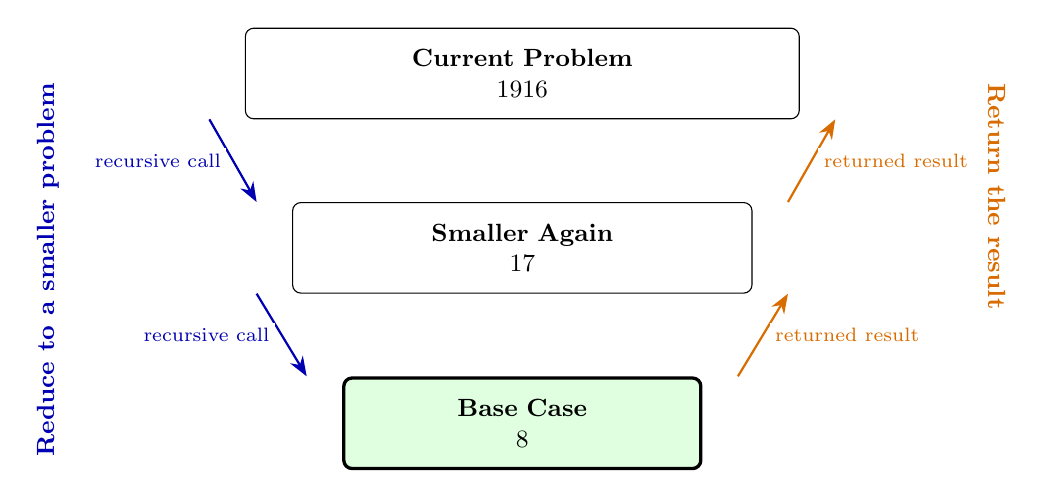
\begin{tikzpicture}[
        problem/.style={
            draw,
            rounded corners=3pt,
            minimum height=1.15cm,
            align=center,
            font=\small
        },
        basecase/.style={
            problem,
            fill=green!12,
            very thick
        },
        callarrow/.style={
            -{Stealth[length=2.5mm]},
            thick,
            blue!70!black
        },
        returnarrow/.style={
            -{Stealth[length=2.5mm]},
            thick,
            orange!85!black
        },
        arrowlabel/.style={
            font=\scriptsize,
            fill=white,
            inner sep=2pt
        },
        node distance=1.05cm
    ]

        % ---------------------------------------------------------------------
        % Progressively smaller problems
        % ---------------------------------------------------------------------

        \node[
            problem,
            text width=6.8cm
        ] (problem1) {
            \textbf{Current Problem}\\
            1916
        };

        \node[
            problem,
            text width=5.6cm,
            below=of problem1
        ] (problem2) {
            \textbf{Smaller Again}\\
            17
        };

        \node[
            basecase,
            text width=4.3cm,
            below=of problem2
        ] (base) {
            \textbf{Base Case}\\
            8
        };

        % ---------------------------------------------------------------------
        % Downward recursive calls
        % ---------------------------------------------------------------------

        \draw[callarrow]
            ($(problem1.south west)+(-0.45,0)$)
            --
            node[arrowlabel, left=2pt] {recursive call}
            ($(problem2.north west)+(-0.45,0)$);

        % \draw[callarrow]
        %     ($(problem2.south west)+(-0.45,0)$)
        %     --
        %     node[arrowlabel, left=2pt] {recursive call}
        %     ($(problem2.north west)+(-0.45,0)$);

        \draw[callarrow]
            ($(problem2.south west)+(-0.45,0)$)
            --
            node[arrowlabel, left=2pt] {recursive call}
            ($(base.north west)+(-0.45,0)$);

        % ---------------------------------------------------------------------
        % Upward returned results
        % ---------------------------------------------------------------------

        \draw[returnarrow]
            ($(base.north east)+(0.45,0)$)
            --
            node[arrowlabel, right=2pt] {returned result}
            ($(problem2.south east)+(0.45,0)$);

        % \draw[returnarrow]
        %     ($(problem2.north east)+(0.45,0)$)
        %     --
        %     node[arrowlabel, right=2pt] {returned result}
        %     ($(problem2.south east)+(0.45,0)$);

        \draw[returnarrow]
            ($(problem2.north east)+(0.45,0)$)
            --
            node[arrowlabel, right=2pt] {returned result}
            ($(problem1.south east)+(0.45,0)$);

        % ---------------------------------------------------------------------
        % Journey labels
        % ---------------------------------------------------------------------

        \node[
            font=\small\bfseries,
            blue!70!black,
            rotate=90,
            left=2.5cm of problem1
        ] {
            Reduce to a smaller problem
        };

        \node[
            font=\small\bfseries,
            orange!85!black,
            rotate=270,
            right=2.5cm of problem1
        ] {
            Return the result
        };

    \end{tikzpicture}

    \caption{Recursive sums: calls repeatedly sum the digits until a value < 9 remain.}
    \label{fig:recursive-decomposition-1}
\end{figure}

\subsection{Inspect the Tests}

Open:

\begin{terminal}
tests/test01_recursive_thinking.cpp
\end{terminal}

The tests are organised from the smallest problems to repeated reduction.

Run the test suite:

\begin{terminal}
make test01
\end{terminal}

At the start, the Digital Root starter implementation simply returns the input.
This means the single-digit cases may already pass while larger values fail.

Use the tests in this order:

\begin{enumerate}
    \item make all single-digit cases pass;
    \item make two-digit reductions pass;
    \item make values requiring repeated reduction pass;
    \item verify the larger values.
\end{enumerate}

Do not attempt to write a complicated solution immediately. Implement the
smallest behaviour required by the next failing test.

\subsection{Implement \mintinline{cpp}{digitalRoot()}}

Open:

\begin{terminal}
src/recursion_exercises.cpp
\end{terminal}

Locate the starter function:

\begin{cppcode}
int digitalRoot(int value)
{
    // TODO: Implement this function recursively.
    return value;
}
\end{cppcode}

Use your answers to the three design questions.

The completed function requires:

\begin{itemize}
    \item a base case for values that are already one digit;
    \item a recursive call using the smaller value created by
          \mintinline{cpp}{digitSum()};
    \item a return value that propagates the final one-digit answer.
\end{itemize}

After each change, run:

\begin{terminal}
make test01
\end{terminal}

Continue until every Digital Root test passes.

\begin{commonerror}
\textbf{Summing the digits only once}

Returning \mintinline{cpp}{digitSum(value)} is not sufficient for values such as
\mintinline{cpp}{1916}:

\begin{cppcode}
digitSum(1916) == 17
\end{cppcode}

The result is still not a single digit.

The smaller problem must be passed back to \mintinline{cpp}{digitalRoot()} so
that the same reasoning is applied again.
\end{commonerror}

\begin{commonerror}
\textbf{Forgetting the stopping condition}

A recursive call must move towards a case that returns without making another
recursive call.

If \mintinline{cpp}{digitalRoot()} calls itself for every input, including
single-digit values, the recursion will not terminate correctly.
\end{commonerror}

\subsection{Verify and Commit}

When all Digital Root tests pass, rebuild and run the complete core suite:

\begin{terminal}
make clean
make
make test01
\end{terminal}

Confirm that your implementation compiles without warnings and that no
previously passing tests have been broken.

Commit your completed Part A work:

\begin{terminal}
git add .
git commit -m "Complete recursive digital root"
git push
\end{terminal}

\subsection{Part A Reflection}

\begin{reflectionbox}
Without looking at your code, explain \mintinline{cpp}{digitalRoot()} using the
three questions:

\begin{enumerate}
    \item What is the base case?
    \item What is the smaller problem?
    \item What result is returned to the waiting call?
\end{enumerate}

Then compare it with the reciprocal-square demonstration.

The calculations are different, but what recursive structure do they share?
\end{reflectionbox}

\subsection{Engineering Takeaway}

\begin{importantnote}
Recursive functions are not patterns to memorise.

Begin by identifying the smallest problem, the smaller version of the current
problem and the work that remains. Once those decisions are clear, the code
often becomes a direct record of the reasoning.
\end{importantnote}

% End of Part A

%%%%%%%%%%%%%%%%%%%%%%%%%%%%%%%%%%%%%%%%%%%%%%%%%%%%%%%%%%%%%%%%%%%%%%%%%%%%%%%%
% Practical 7 -- Parts B and C
%%%%%%%%%%%%%%%%%%%%%%%%%%%%%%%%%%%%%%%%%%%%%%%%%%%%%%%%%%%%%%%%%%%%%%%%%%%%%%%%

\section{Part B -- Recognising Recursive Structures}

\begin{learningoutcomes}
By the end of this part, you should be able to:

\begin{itemize}
    \item recognise a familiar problem as a collection of smaller problems of
          the same kind;
    \item apply the three recursive-design questions without relying on C++
          syntax;
    \item explain what information one recursive search must return to the
          search that called it;
    \item identify when you need to revisit Part A or ask for help.
\end{itemize}
\end{learningoutcomes}

\begin{infobox}[Estimated Effort]
Estimated time: \textbf{5--10 minutes}
\end{infobox}

Part A used numerical examples because the smaller problem was easy to expose.
Recursion is much more useful, however, when the structure of the real problem
already contains smaller versions of itself.

You will now consider a task you may already perform without thinking of it as
an algorithm.

\subsection{The Missing File}

Imagine that you know the name of a file but cannot remember where it was
saved.

You begin inside the \texttt{Documents} folder. The folder hierarchy contains
several areas of work, each of which may contain further folders and files.

\begin{figure}[htbp]
    \centering
    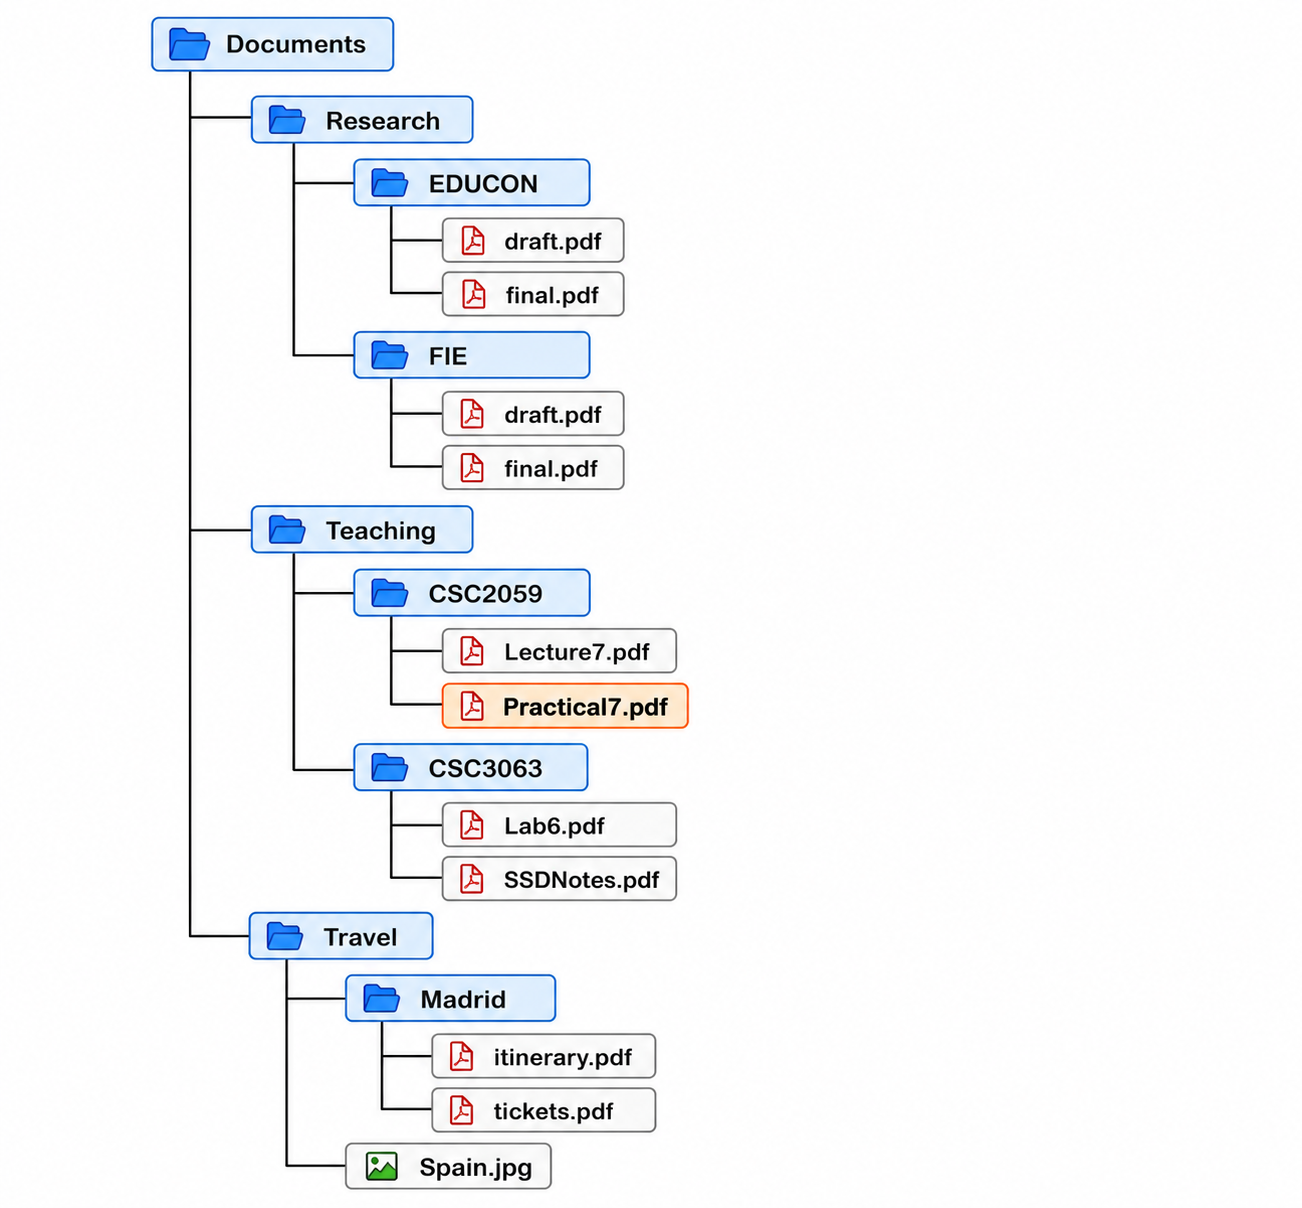
\includegraphics[width=0.75\textwidth,keepaspectratio]{../../../assets/figures/practical07/file_tree.png}
    \caption{A simplified document collection containing folders and files.}
    \label{fig:codument-tree}
\end{figure}

\begin{engineeringquestion}
How would you search the hierarchy systematically for
\texttt{Practical7.pdf} if you did not already know its location?
\end{engineeringquestion}

\begin{infobox}[Plan Before Continuing]
Take a moment to plan the order in which you would explore the hierarchy.

Use whichever medium best supports your reasoning:

\begin{itemize}
    \item sketch the order on paper;
    \item write a short sequence in a text file;
    \item use a scratch file in Visual Studio Code;
    \item or reason through it mentally.
\end{itemize}

The medium does not matter. The important part is that you make the search
process explicit before reading on.
\end{infobox}

A systematic search might begin by inspecting the current folder, then
searching each subfolder in turn.

The important observation is not whether you can visually spot the file. It is
whether your search process still works when the hierarchy is too large to
inspect at a glance.

\clearpage

\subsection{Apply the Three Questions Again}

Return to the three questions from Part A.

\begin{enumerate}
    \item What is the smallest search problem?
    \item How does the current search create a smaller problem?
    \item What information must the smaller search return?
\end{enumerate}

For a folder search:

\begin{itemize}
    \item the current folder may contain the target;
    \item each subfolder represents a smaller search problem;
    \item each smaller search needs to report whether the target was found.
\end{itemize}

If one subfolder reports success, that result can be returned to the search
that asked for it. If not, the current search continues with the remaining
subfolders.


\begin{reflectionbox}
Without looking back at Part A, answer these questions:

\begin{enumerate}
    \item What was the smallest search problem?
    \item What made each search smaller?
    \item What information did each search need to return?
\end{enumerate}

If these questions were difficult to answer, revisit the three-question method
in Part A or ask a demonstrator for help before moving on.

The next part assumes that this reasoning is secure.
\end{reflectionbox}

\subsection{Engineering Takeaway}

\begin{importantnote}
Recursive thinking is not limited to mathematical functions.

Whenever part of a problem has the same structure as the whole problem, the
same design process may apply.
\end{importantnote}


\section{Part C -- Constructing and Searching a Binary Tree}

\begin{learningoutcomes}
By the end of this part, you should be able to:

\begin{itemize}
    \item explain how a binary tree simplifies a more general hierarchy;
    \item identify roots, child nodes, leaves and subtrees;
    \item construct a binary tree using dynamically allocated nodes;
    \item navigate the tree manually using child pointers;
    \item implement a recursive search using public tests;
    \item explain why deleting the root deletes the complete tree.
\end{itemize}
\end{learningoutcomes}

\begin{infobox}[Estimated Effort]
Estimated time: \textbf{35--45 minutes}
\end{infobox}

The folder hierarchy in Part B allowed each folder to contain any number of
children. That is realistic, but it introduces more implementation detail than
we need while learning the underlying recursive ideas.

Engineers often simplify a real system temporarily so that its essential
behaviour is easier to study.

\begin{infobox}[Engineering Simplification]
For the next part, every node will be allowed at most two children.

This is an artificial restriction. Its purpose is to help you study recursive
structures without introducing unnecessary representation complexity.
\end{infobox}

\subsection{From a Hierarchy to a Binary Tree}

Consider the following simplified folder hierarchy:

\begin{figure}[htbp]
    \centering

    \begin{forest}
        for tree={
            grow'=south,
            parent anchor=south,
            child anchor=north,
            edge={
                draw=black!45,
                line width=0.7pt
            },
            font=\small,
            align=center,
            l sep=11mm,
            s sep=4mm,
            inner xsep=5pt,
            inner ysep=4pt
        },
        folder/.style={
            draw=blue!65!black,
            fill=blue!9,
            rounded corners=3pt,
            font=\small\bfseries
        },
        [\faFolder\ Documents, folder
            [\faFolder\ Teaching, folder
                [\faFolder\ CSC3063, folder]
                [\faFolder\ CSC2059, folder]
            ]
            [\faFolder\ Research, folder
                [\faFolder\ FIE, folder]
                [\faFolder\ EDUCON, folder]
            ]
        ]
    \end{forest}

    \medskip

    \caption{A simplified document collection containing folders and files.}
    \label{fig:document-collection}
\end{figure}


This structure is a \textbf{binary tree}: each node has at most two children.

The terminology used throughout this practical is:

\begin{center}
\begin{tabular}{p{0.22\textwidth} p{0.66\textwidth}}
\toprule
\textbf{Term} & \textbf{Meaning} \\
\midrule
Root & The first node in the tree. Here, it is
\texttt{Documents}. \\
Node & One stored item together with links to its children. \\
Child & A node immediately below another node. \\
Leaf & A node with no children. \\
Subtree & A node together with every node below it. \\
Empty tree & A tree represented by no node at all. \\
\bottomrule
\end{tabular}
\end{center}

Notice that \texttt{Research} is both:

\begin{itemize}
    \item the left child of \texttt{Documents}; and
    \item the root of a smaller tree containing \texttt{Research},
          \texttt{EDUCON} and \texttt{FIE}.
\end{itemize}

That second interpretation is what makes the structure recursive.

\begin{engineeringquestion}
What information must one node store if it is allowed at most two children?
\end{engineeringquestion}

A suitable representation needs:

\begin{itemize}
    \item the stored item;
    \item a pointer to the left child;
    \item a pointer to the right child.
\end{itemize}

\subsection{Inspect \mintinline{text}{TreeNode.h}}

Open:

\begin{terminal}
include/TreeNode.h
\end{terminal}

The supplied class template defines one node in the tree.

Locate these members:

\begin{cppcode}
T item;
TreeNode<T>* leftTree;
TreeNode<T>* rightTree;
\end{cppcode}

The type parameter \mintinline{cpp}{T} allows the tree to store different kinds
of data. In this part, the stored items are strings representing folder names.

The child pointers are initialised to \mintinline{cpp}{nullptr} when no child is
provided.

\begin{tipbox}
Read \mintinline{cpp}{nullptr} as ``there is no subtree here.''

An empty left or right child is not an error. It is the point where a recursive
tree algorithm eventually stops.
\end{tipbox}

\subsection{Ownership and Recursive Destruction}

The destructor is deliberately small:

\begin{cppcode}
TreeNode<T>::~TreeNode()
{
    delete leftTree;
    delete rightTree;
}
\end{cppcode}

Deleting one node therefore deletes both smaller trees beneath it. Each child
repeats the same process for its own children.

As a result:

\begin{cppcode}
delete tree;
\end{cppcode}

deletes the root and every node beneath it.

This is another recursive algorithm, even though it contains no explicit call
to the destructor by name.

\begin{importantnote}
A \mintinline{cpp}{TreeNode} owns its left and right subtrees.

Every child attached to the tree must therefore be created dynamically using
\mintinline{cpp}{new}, so that the recursive destructor can safely release it
using \mintinline{cpp}{delete}.
\end{importantnote}

\begin{commonerror}
\textbf{Creating child nodes on the stack}

The following is incorrect:

\begin{cppcode}
TreeNode<std::string> research("Research");
tree->leftTree = &research;
\end{cppcode}

The root now points to a stack object. Later, deleting the root eventually
attempts:

\begin{cppcode}
delete &research;
\end{cppcode}

But \mintinline{cpp}{research} was not created using
\mintinline{cpp}{new}. This is undefined behaviour.

What could happen?

It may appear to work. It may crash. It may corrupt memory. It may summon some
eldritch horror.

Once execution enters undefined behaviour, the C++ standard makes no promises
about what happens next.
\end{commonerror}

\subsection{Build the Tree Using Tests}

Open:

\begin{terminal}
tests/test02_binary_tree_construction.cpp
\end{terminal}

The tests reveal the tree one level at a time:

\begin{enumerate}
    \item the root is \texttt{Documents};
    \item its children are \texttt{Research} and \texttt{Teaching};
    \item \texttt{Research} contains \texttt{EDUCON} and \texttt{FIE};
    \item \texttt{Teaching} contains \texttt{CSC2059} and \texttt{CSC3063};
    \item the lowest-level nodes are leaves.
\end{enumerate}

Run only the construction tests:

\begin{terminal}
make test02
\end{terminal}

Open:

\begin{terminal}
src/tree_exercises.cpp
\end{terminal}

Locate:

\begin{cppcode}
TreeNode<std::string>* buildFileTree()
\end{cppcode}

The starter implementation creates only the root. Extend it gradually.

A typical allocation looks like:

\begin{cppcode}
TreeNode<std::string>* research =
    new TreeNode<std::string>("Research");
\end{cppcode}

A child is attached using:

\begin{cppcode}
tree->leftTree = research;
\end{cppcode}

Do not construct the entire tree in one untested burst.

Use the TDD rhythm:

\begin{enumerate}
    \item run \mintinline{text}{make test02};
    \item read the next failing test;
    \item add only the nodes and links required by that test;
    \item run the test again;
    \item continue until every construction test passes.
\end{enumerate}

\begin{tipbox}
Keep the diagram visible while constructing the tree.

For every assignment, identify:

\begin{itemize}
    \item the parent node;
    \item whether the child belongs on the left or right;
    \item whether the child itself requires further children.
\end{itemize}
\end{tipbox}

\begin{commonerror}
\textbf{Creating the right nodes but attaching them incorrectly}

The labels may all exist while the tree shape is still wrong.

For example, swapping \texttt{Research} and \texttt{Teaching} creates a
different tree even though every folder name is present.

The tests check relationships, not merely values.
\end{commonerror}

\subsection{Verify the Leaves}

The final construction test checks that:

\begin{itemize}
    \item \texttt{EDUCON};
    \item \texttt{FIE};
    \item \texttt{CSC2059}; and
    \item \texttt{CSC3063}
\end{itemize}

have no children.

This matters because leaves are where tree algorithms encounter empty left and
right subtrees.

A leaf still exists as a node. Its children do not.

\begin{reflectionbox}
For the completed tree:

\begin{enumerate}
    \item Which node is the root?
    \item Which nodes are leaves?
    \item What is the left subtree of \texttt{Documents}?
    \item What is the right subtree of \texttt{Research}?
\end{enumerate}
\end{reflectionbox}

\subsection{Navigate the Completed Tree}

Once all construction tests pass, run:

\begin{terminal}
make run-example02
\end{terminal}

The example pauses before showing the result of several pointer expressions.

For each expression:

\begin{enumerate}
    \item predict the output using the diagram;
    \item identify the path from the root;
    \item press Enter to observe the result.
\end{enumerate}

For example:

\begin{cppcode}
tree->leftTree->item
\end{cppcode}

means:

\begin{quote}
Begin at the root, move to the left child, then read its item.
\end{quote}

A longer expression such as:

\begin{cppcode}
tree->rightTree->leftTree->item
\end{cppcode}

means:

\begin{quote}
Begin at the root, move right, then left, then read the item.
\end{quote}

\begin{engineeringquestion}
Which expressions reach:

\begin{itemize}
    \item \texttt{EDUCON};
    \item \texttt{FIE};
    \item \texttt{CSC2059};
    \item \texttt{CSC3063}?
\end{itemize}
\end{engineeringquestion}

The example ends by deleting the root. Observe that no separate
\mintinline{cpp}{delete} calls are required for the child nodes.

\subsection{Experience the Limitation}

Manual navigation works only when the exact path is already known.

For example:

\begin{cppcode}
tree->rightTree->leftTree->item
\end{cppcode}

can retrieve \texttt{CSC2059} because the programmer already knows where it is.

That expression is not a search algorithm. It is a hard-coded route.

\begin{engineeringquestion}
What should the program do if it knows the target name but not whether the item
is in the root, left subtree or right subtree?
\end{engineeringquestion}

This is the same problem you considered in Part B, now expressed using the
binary-tree structure.

\subsection{Design the Recursive Search}

The initial search contract is:

\begin{cppcode}
bool search(
    const TreeNode<std::string>* tree,
    const std::string& value
);
\end{cppcode}

It asks:

\begin{quote}
Does the tree rooted at \mintinline{cpp}{tree} contain
\mintinline{cpp}{value}?
\end{quote}

Apply the three questions.

\begin{center}
\begin{tabular}{p{0.34\textwidth} p{0.54\textwidth}}
\toprule
\textbf{Question} & \textbf{Answer for Tree Search} \\
\midrule
What is the smallest problem? &
An empty tree contains no matching item. \\
How does the problem become smaller? &
Search the left subtree or the right subtree. \\
What work remains? &
Return whether the current item matches or either smaller search succeeds. \\
\bottomrule
\end{tabular}
\end{center}

This leads to the behavioural structure:

\begin{enumerate}
    \item if the tree is empty, return \mintinline{cpp}{false};
    \item if the current item matches, return \mintinline{cpp}{true};
    \item otherwise search the left subtree;
    \item if necessary, search the right subtree;
    \item return \mintinline{cpp}{false} only when no search succeeds.
\end{enumerate}


\subsection{Let the Tests Reveal the Algorithm}

Open:

\begin{terminal}
tests/test03_recursive_tree_search.cpp
\end{terminal}

Run only these tests:

\begin{terminal}
make test03
\end{terminal}

The tests are ordered deliberately.

\subsubsection*{Step 1: Empty Tree}

The first test checks:

\begin{cppcode}
search(nullptr, "CSC2059")
\end{cppcode}

This establishes the base case.

\subsubsection*{Step 2: Current Node}

The next test searches for \texttt{Documents}. The answer is available at the
current node and requires no recursive call.

\subsubsection*{Step 3: Left Subtree}

The next tests search for \texttt{Research}, \texttt{EDUCON} and \texttt{FIE}.
A solution that checks only the immediate child is not enough. The search must
work at any depth.

\subsubsection*{Step 4: Right Subtree}

The next tests search for \texttt{Teaching}, \texttt{CSC2059} and
\texttt{CSC3063}. These expose an implementation that searches only the left
side.

\subsubsection*{Step 5: Missing Values}

The final tests use values that do not appear anywhere in the tree. A correct
search must reach empty subtrees safely and propagate
\mintinline{cpp}{false} back to the root.

\begin{importantnote}
The starter implementation returns \mintinline{cpp}{false}.

This means the empty-tree and missing-value cases may pass before the search is
complete. A few green tests do not mean that the algorithm is finished.

Work through the test cases in the order shown in the guide.
\end{importantnote}

\subsection{Implement \mintinline{cpp}{search()}}

Open:

\begin{terminal}
src/tree_algorithms.cpp
\end{terminal}

Locate the starter function.

Implement one behaviour at a time and rerun:

\begin{terminal}
make test03
\end{terminal}

A useful expanded structure is:

\begin{itemize}
    \item handle \mintinline{cpp}{nullptr};
    \item compare the current item;
    \item store or return the left-subtree result;
    \item search the right subtree when required;
    \item combine the returned values.
\end{itemize}

Do not copy a finished search algorithm from another source. The purpose of
the tests is to help you assemble it from behaviours you understand.

\begin{commonerror}
\textbf{Dereferencing before checking for an empty tree}

The following is unsafe when \mintinline{cpp}{tree} is
\mintinline{cpp}{nullptr}:

\begin{cppcode}
if (tree->item == value)
\end{cppcode}

Check the empty-tree base case before accessing any members.
\end{commonerror}

\begin{commonerror}
\textbf{Searching only one subtree}

A recursive call to the left subtree may pass several tests while still
ignoring the entire right side of the tree.

The return value must account for both smaller search problems.
\end{commonerror}

\begin{commonerror}
\textbf{Checking only the immediate children}

Expressions such as:

\begin{cppcode}
tree->leftTree->item == value
\end{cppcode}

do not search a subtree. They inspect only one known node.

The recursive call must receive the child pointer so that the same algorithm is
applied to every node below it.
\end{commonerror}

\subsection{Verify and Commit}

When every search test passes, run:

\begin{terminal}
make test02
make test03
\end{terminal}

The construction tests remain valuable regression tests. The search algorithm
depends on the tree being constructed correctly.

Commit your work:

\begin{terminal}
git add .
git commit -m "Build and search binary tree"
git push
\end{terminal}

\subsection{Part C Reflection}

\begin{reflectionbox}
Compare manual navigation with recursive search.

\begin{enumerate}
    \item What information did the hard-coded pointer path assume?
    \item What does the recursive search discover for itself?
    \item Where is the base case in the tree?
    \item What value travels back towards the root?
\end{enumerate}
\end{reflectionbox}

\subsection{Engineering Takeaway}

\begin{importantnote}
A binary tree is recursive because each child is the root of another, smaller
binary tree.

Once that structure is recognised, the search algorithm follows the same
three-question process used for the numerical examples in Part A.
\end{importantnote}

% End of Parts B and C

%%%%%%%%%%%%%%%%%%%%%%%%%%%%%%%%%%%%%%%%%%%%%%%%%%%%%%%%%%%%%%%%%%%%%%%%%%%%%%%%
% Practical 7 -- Part D
%%%%%%%%%%%%%%%%%%%%%%%%%%%%%%%%%%%%%%%%%%%%%%%%%%%%%%%%%%%%%%%%%%%%%%%%%%%%%%%%

\section{Part D -- Reusing and Generalising the Recursive Pattern}

\begin{learningoutcomes}
By the end of this part, you should be able to:

\begin{itemize}
    \item calculate the depth of a binary tree recursively;
    \item explain why both subtrees must be measured;
    \item combine recursive results using the structure of the problem;
    \item distinguish an algorithm that depends on stored values from one that
          depends only on tree shape;
    \item use a guided compile failure to identify a limitation in an
          interface;
    \item refactor a concrete recursive function into a reusable function
          template;
    \item explain why template implementations must be visible in a header
          file.
\end{itemize}
\end{learningoutcomes}

\begin{infobox}[Estimated Effort]
Estimated time: \textbf{25--35 minutes}
\end{infobox}

The search algorithm in Part C answered one question:

\begin{quote}
Does this tree contain a particular item?
\end{quote}

You will now answer a different question using the same recursive structure:

\begin{quote}
How deep is this tree?
\end{quote}

The purpose is not to memorise another recursive function. It is to recognise
which parts of the earlier algorithm remain stable and which parts change when
the required result changes.

\begin{importantnote}
The guiding idea for this part is:

\begin{center}
\textbf{Keep the recursion. Change the work.}
\end{center}
\end{importantnote}

\subsection{Measuring a Tree}

The \textbf{depth} of a tree is the number of nodes on the longest path from the
root to a leaf.

For the simplified file tree:

\begin{figure}[htbp]
    \centering

    \begin{forest}
    for tree={
        grow'=south,
        parent anchor=south,
        child anchor=north,
        edge={
            draw=black!45,
            line width=0.7pt
        },
        font=\small,
        align=center,
        l sep=11mm,
        s sep=4mm,
        inner xsep=5pt,
        inner ysep=4pt,
        rounded corners=3pt,
        font=\small\bfseries
    },
    level1/.style={
        draw=blue!70!black,
        fill=blue!12
    },
    level2/.style={
        draw=cyan!60!black,
        fill=cyan!10
    },
    level3/.style={
        draw=green!55!black,
        fill=green!10
    }
    [
        \faFolder\ Documents,
        level1,
        label={
            [font=\small\bfseries, text=blue!70!black]
            right:Level 1
        }
        [
            \faFolder\ Teaching,
            level2,
            label={
                [font=\small\bfseries, text=cyan!55!black]
                right:Level 2
            }
            [
                \faFolder\ CSC3063,
                level3,
                label={
                    [font=\small\bfseries, text=green!45!black]
                    right:Level 3
                }
            ]
            [
                \faFolder\ CSC2059,
                level3
            ]
        ]
        [
            \faFolder\ Research,
            level2
            [
                \faFolder\ FIE,
                level3
            ]
            [
                \faFolder\ EDUCON,
                level3
            ]
        ]
    ]
\end{forest}

    \medskip
    \medskip

\begin{center}
    \colorbox{orange!12}{%
        \strut\textbf{\textcolor{orange!85!black}{Tree depth = 3}}%
    }
\end{center}

    \caption{The depth of the simplified binary tree is three levels.}
    \label{fig:binary-tree-depth}
\end{figure}

the longest root-to-leaf path contains three nodes:

\[
\texttt{Documents}
\rightarrow
\texttt{Research}
\rightarrow
\texttt{EDUCON}
\]

Therefore, the tree has depth \(3\).

An empty tree contains no nodes, so its depth is defined as \(0\).

A tree containing only one node has depth \(1\).

\begin{engineeringquestion}
How can the depth of the whole tree be calculated if the depths of its left
and right subtrees are already known?
\end{engineeringquestion}

The current node adds one level above whichever subtree is deeper:

\[
\operatorname{depth}(\text{tree})
=
1+
\max
\left(
\operatorname{depth}(\text{left}),
\operatorname{depth}(\text{right})
\right)
\]

The formula contains the same recursive structure seen earlier:

\begin{itemize}
    \item measure a smaller left subtree;
    \item measure a smaller right subtree;
    \item combine the returned results;
    \item include the current node.
\end{itemize}

\subsection{Apply the Three Questions}

Use the same design method once again.

\begin{center}
\begin{tabular}{p{0.34\textwidth} p{0.54\textwidth}}
\toprule
\textbf{Question} & \textbf{Answer for Tree Depth} \\
\midrule
What is the smallest problem? &
An empty tree has depth \(0\). \\
How does the problem become smaller? &
Measure the left and right subtrees. \\
What work remains? &
Choose the larger returned depth and add \(1\) for the current node. \\
\bottomrule
\end{tabular}
\end{center}

Compare this with recursive search.

Search could stop as soon as one branch reported success. Depth cannot assume
that either side is deepest. It must measure both subtrees before combining
their answers.

\begin{reflectionbox}
Why would the following strategy be unreliable?

\begin{quote}
Follow the left subtree until a leaf is reached and use that length as the
depth.
\end{quote}

Sketch or imagine a tree for which the deepest path lies on the right.
\end{reflectionbox}

\subsection{Recognise the Recursive Skeleton}

The search algorithm contained these decisions:

\begin{itemize}
    \item stop at an empty tree;
    \item inspect the current node;
    \item recurse into smaller subtrees;
    \item combine returned Boolean values.
\end{itemize}

The depth algorithm contains:

\begin{itemize}
    \item stop at an empty tree;
    \item recurse into smaller subtrees;
    \item combine returned integer values;
    \item add the current node.
\end{itemize}

The returned type and combination rule have changed. The structural recursion
has not.

% =============================================================================
% Figure Placeholder
% =============================================================================
% TODO: Insert a side-by-side "Keep the recursion; change the work" figure.
%
% Shared skeleton:
%
%   empty tree?
%       |
%       v
%   solve left subtree
%   solve right subtree
%       |
%       v
%   combine results
%
% Search combination:
%   current match OR left result OR right result
%
% Depth combination:
%   1 + max(left depth, right depth)
%
% Use the same tree node and arrow language as earlier figures.
% =============================================================================

\subsection{Inspect the Depth Interface}

Open:

\begin{terminal}
include/tree_algorithms.h
\end{terminal}

Locate the starter function:

\begin{cppcode}
template <typename T>
int depth(const TreeNode<T>* tree)
{
    // TODO: Implement this function recursively.
    return 0;
}
\end{cppcode}

Unlike the first version of \mintinline{cpp}{search()}, the depth function is
already a template.

This is appropriate because depth does not inspect
\mintinline{cpp}{tree->item}. It depends only on:

\begin{itemize}
    \item whether the current node exists;
    \item the shape of the left subtree;
    \item the shape of the right subtree.
\end{itemize}

The same implementation can therefore measure:

\begin{cppcode}
TreeNode<int>
TreeNode<std::string>
\end{cppcode}

without knowing anything about the stored type.

\begin{importantnote}
The full starter definition appears in the header, not merely the function
prototype.

When a compiler encounters \mintinline{cpp}{depth<int>()} or
\mintinline{cpp}{depth<std::string>()}, it needs to see the complete template
definition so that it can generate the required concrete function.
\end{importantnote}

\subsection{Let Different Tree Shapes Guide the Implementation}

Open:

\begin{terminal}
tests/test04_tree_depth.cpp
\end{terminal}

The tests deliberately use several shapes:

\begin{enumerate}
    \item an empty tree;
    \item a single-node tree;
    \item the balanced file tree;
    \item a left-skewed tree;
    \item a right-skewed tree;
    \item an uneven tree.
\end{enumerate}

Run only the depth tests:

\begin{terminal}
make test04
\end{terminal}

The starter implementation returns \(0\), so the empty-tree test should pass
while non-empty cases fail.

Work through the tests in order.

\subsubsection*{Step 1: Empty Tree}

The first test establishes:

\begin{cppcode}
depth(nullptr) == 0
\end{cppcode}

This is the base case.

\subsubsection*{Step 2: One Node}

A non-empty node contributes one level even when both children are empty.

\subsubsection*{Step 3: Balanced Tree}

The shared file tree confirms that the function can measure both branches of a
regular structure.

\subsubsection*{Step 4: Skewed Trees}

The left- and right-skewed tests prevent the implementation from assuming that
the deepest path always lies on a particular side.

\subsubsection*{Step 5: Uneven Tree}

The final test checks that both returned values are compared and that the
larger result is retained.

\subsection{Implement \mintinline{cpp}{depth()}}

Complete the starter definition in:

\begin{terminal}
include/tree_algorithms.h
\end{terminal}

Use an expanded implementation while developing the function:

\begin{itemize}
    \item check the empty-tree base case;
    \item calculate the left depth;
    \item calculate the right depth;
    \item select the larger result;
    \item add one for the current node.
\end{itemize}

You may use \mintinline{cpp}{std::max()} if the appropriate standard header is
included, or use a clear conditional expression.

After each change, run:

\begin{terminal}
make test04
\end{terminal}

\begin{commonerror}
\textbf{Adding one in the empty-tree case}

If an empty tree returns \(1\), every non-empty depth will be one level too
large.

The value \(1\) belongs to the current existing node. An empty tree contains no
current node.
\end{commonerror}

\begin{commonerror}
\textbf{Adding the subtree depths together}

The depth is the length of one longest path. It is not the total number of
levels across both branches.

The recursive results must be compared, not summed.
\end{commonerror}

\begin{commonerror}
\textbf{Measuring only one side}

A solution that always returns the left depth may pass balanced and left-skewed
examples while failing right-skewed or uneven trees.

The tests use varied shapes specifically to expose this assumption.
\end{commonerror}

\subsection{Verify the Reused Pattern}

When all depth tests pass, compare the structure of
\mintinline{cpp}{depth()} with \mintinline{cpp}{search()}.

Complete the following comparison in your own words:

\begin{center}
\begin{tabular}{p{0.25\textwidth} p{0.3\textwidth} p{0.3\textwidth}}
\toprule
& \textbf{Search} & \textbf{Depth} \\
\midrule
Base case &
Empty tree returns false. &
Empty tree returns zero. \\
Smaller problems &
Search left and right. &
Measure left and right. \\
Combination &
Use Boolean OR. &
Use the larger depth and add one. \\
\bottomrule
\end{tabular}
\end{center}

\begin{reflectionbox}
Which parts of these algorithms are caused by the binary-tree structure?

Which parts are caused by the particular question being answered?
\end{reflectionbox}

\subsection{A Limitation in the Search Interface}

The initial search function was designed for the concrete problem in Part C:

\begin{cppcode}
bool search(
    const TreeNode<std::string>* tree,
    const std::string& value
);
\end{cppcode}

It searches a tree of folder names.

Now consider an integer tree:

\begin{cppcode}
TreeNode<int>* tree = new TreeNode<int>(10);
\end{cppcode}

The recursive reasoning is unchanged:

\begin{itemize}
    \item an empty tree does not contain the target;
    \item compare the target with the current item;
    \item search the left subtree;
    \item search the right subtree.
\end{itemize}

Only the stored type has changed.

\begin{engineeringquestion}
Does the search algorithm genuinely depend on strings, or is the function
interface unnecessarily restrictive?
\end{engineeringquestion}

The concrete interface has now exposed a code smell:

\begin{quote}
The implementation expresses a more general algorithm than its public
contract allows.
\end{quote}

This is the right moment to generalise it.

\subsection{Observe the Guided Compile Failure}

The repository contains:

\begin{terminal}
tests/test05_generic_tree_search.cpp
\end{terminal}

This test file is not part of the normal core suite yet. Run its dedicated
target:

\begin{terminal}
make test-generic-search
\end{terminal}

Before the refactor, compilation should fail.

The error may report that no matching \mintinline{cpp}{search()} function can
accept arguments similar to:

\begin{cppcode}
TreeNode<int>*
int
\end{cppcode}

This failure is expected.

The new test has revealed that the current function contract accepts only:

\begin{cppcode}
TreeNode<std::string>*
const std::string&
\end{cppcode}

\begin{importantnote}
This is a guided failure, not a debugging puzzle.

The test is deliberately incompatible with the initial interface. Its purpose
is to make the limitation visible before you change the code.
\end{importantnote}

\subsection{Plan the Refactoring}

The current declaration is:

\begin{cppcode}
bool search(
    const TreeNode<std::string>* tree,
    const std::string& value
);
\end{cppcode}

The target generic form is:

\begin{cppcode}
template <typename T>
bool search(
    const TreeNode<T>* tree,
    const T& value
);
\end{cppcode}

The body of the algorithm does not need a new recursive strategy.

The refactor changes:

\begin{enumerate}
    \item the concrete stored type into a type parameter;
    \item the concrete target type into the same type parameter;
    \item the location of the implementation.
\end{enumerate}

The recursive decisions remain unchanged.

\subsection{Move the Implementation into the Header}

The concrete \mintinline{cpp}{search()} implementation currently lives in:

\begin{terminal}
src/tree_algorithms.cpp
\end{terminal}

Once \mintinline{cpp}{search()} becomes a template, the compiler must be able to
see the complete definition when it encounters each required type.

Therefore:

\begin{enumerate}
    \item add the template definition to
          \mintinline{text}{include/tree_algorithms.h};
    \item remove the old concrete definition from
          \mintinline{text}{src/tree_algorithms.cpp};
    \item keep the recursive body logically unchanged.
\end{enumerate}

\begin{commonerror}
\textbf{Templating only the declaration}

The following is not enough:

\begin{cppcode}
template <typename T>
bool search(
    const TreeNode<T>* tree,
    const T& value
);
\end{cppcode}

If the definition remains hidden in a separate source file, the compiler may
accept each use but the linker cannot find generated versions such as
\mintinline{cpp}{search<int>()}.

For this practical, keep the complete template implementation in the header.
\end{commonerror}

\subsection{Resolve String-Literal Calls}

After converting \mintinline{cpp}{search()} into a template, calls such as:

\begin{cppcode}
search(tree, "Documents")
\end{cppcode}

may fail template argument deduction.

The first argument implies:

\begin{cppcode}
T = std::string
\end{cppcode}

while the string literal has a character-array type rather than
\mintinline{cpp}{std::string}.

Where required in the existing string-search tests, make the target type
explicit:

\begin{cppcode}
search(tree, std::string("Documents"))
\end{cppcode}

Do this only where the compiler requires it. The purpose is to make both
arguments agree on the same template type.

\begin{tipbox}
Template argument deduction happens before the compiler applies some ordinary
conversions.

An explicit \mintinline{cpp}{std::string(...)} removes the disagreement without
changing the meaning of the test.
\end{tipbox}

\subsection{Run Both Old and New Tests}

After the refactor, run:

\begin{terminal}
make test03
make test-generic-search
\end{terminal}

The original string tests are regression tests. They confirm that the existing
behaviour survived the generalisation.

The new integer tests confirm the expanded capability.

A successful refactor therefore satisfies both:

\begin{quote}
The function still searches folder-name trees correctly.
\end{quote}

and:

\begin{quote}
The same function now searches integer trees.
\end{quote}

Once the dedicated generic-search target passes, follow the supplied Makefile
instruction to add the new test to the normal regression suite, if directed by
your repository version.

\subsection{Review the Design Evolution}

The search algorithm has moved through two stages.

\subsubsection*{Stage 1: Concrete Engineering Problem}

\begin{cppcode}
bool search(
    const TreeNode<std::string>* tree,
    const std::string& value
);
\end{cppcode}

This interface was appropriate when the immediate problem was searching folder
names.

\subsubsection*{Stage 2: Earned Generalisation}

\begin{cppcode}
template <typename T>
bool search(
    const TreeNode<T>* tree,
    const T& value
);
\end{cppcode}

The integer-tree requirement demonstrated that the recursive algorithm did not
depend on strings.

The template now solves an experienced limitation rather than adding
generality in advance.

\begin{reflectionbox}
Why was the concrete string version a reasonable starting point?

What new evidence justified converting it into a template?

How much of the recursive function body changed during the refactor?
\end{reflectionbox}

\subsection{Verify and Commit}

Run the relevant tests together:

\begin{terminal}
make test03
make test04
make test-generic-search
\end{terminal}

Confirm that:

\begin{itemize}
    \item string search still works;
    \item integer search now works;
    \item depth works for integer and string trees;
    \item the project compiles without warnings.
\end{itemize}

Commit your completed Part D work:

\begin{terminal}
git add .
git commit -m "Generalise recursive tree algorithms"
git push
\end{terminal}

\subsection{Part D Reflection}

\begin{reflectionbox}
Consider the phrase:

\begin{center}
\textbf{Keep the recursion. Change the work.}
\end{center}

Explain how it applies to:

\begin{itemize}
    \item recursive search;
    \item tree depth;
    \item the refactoring from string search to generic search.
\end{itemize}

Which changes affected the recursive structure, and which affected only the
operation performed at each node?
\end{reflectionbox}

\subsection{Engineering Takeaway}

\begin{importantnote}
Reusable algorithms emerge when we separate the shape of a problem from the
particular work performed on its data.

The binary-tree structure determined how recursion moved. Search and depth
changed what was returned and how results were combined. The template
refactoring then removed a type restriction that the algorithm never truly
needed.
\end{importantnote}

% End of Part D
%%%%%%%%%%%%%%%%%%%%%%%%%%%%%%%%%%%%%%%%%%%%%%%%%%%%%%%%%%%%%%%%%%%%%%%%%%%%%%%%
% Practical 7 -- Part E and Wrap-up
%%%%%%%%%%%%%%%%%%%%%%%%%%%%%%%%%%%%%%%%%%%%%%%%%%%%%%%%%%%%%%%%%%%%%%%%%%%%%%%%

\section{Part E -- Returning to the Real World}

\begin{learningoutcomes}
By the end of this part, you should be able to:

\begin{itemize}
    \item explain why the binary-tree restriction was useful but not essential;
    \item compare recursive search over two children with recursive search over
          an arbitrary number of children;
    \item identify which parts of the algorithm belong to the recursive idea
          and which belong to the data representation;
    \item recognise transfer of learning from one recursive structure to
          another.
\end{itemize}
\end{learningoutcomes}

\begin{infobox}[Estimated Effort]
Estimated time: \textbf{5--10 minutes}
\end{infobox}

At the beginning of this practical, you considered a realistic folder
hierarchy. A folder could contain several subfolders, and the search strategy
was expressed in ordinary language.

In Part C, that hierarchy was deliberately simplified. Each node was allowed
at most two children so that the recursive structure could be represented using:

\begin{cppcode}
leftTree
rightTree
\end{cppcode}

That simplification made construction, navigation and testing easier.

It is now time to return to the original question.

\begin{engineeringquestion}
Was the binary-tree restriction actually necessary for recursive search?
\end{engineeringquestion}

\subsection{Compare the Two Search Problems}

For a binary tree, the recursive search considered:

\begin{itemize}
    \item the current node;
    \item the left subtree;
    \item the right subtree.
\end{itemize}

Conceptually:

\begin{cppcode}
if the current node matches
    return true

search the left subtree
search the right subtree
\end{cppcode}

For a more general folder hierarchy, a folder may contain any number of
subfolders.

Conceptually:

\begin{cppcode}
if the current folder matches
    return true

for each child folder
    search that child
\end{cppcode}

The way children are visited has changed. The recursive call has not.

\begin{importantnote}
The algorithm was never fundamentally about having exactly two children.

The binary tree was a simplified model that made the recursive structure easier
to study.
\end{importantnote}


\begin{figure}[htbp]
    \centering
    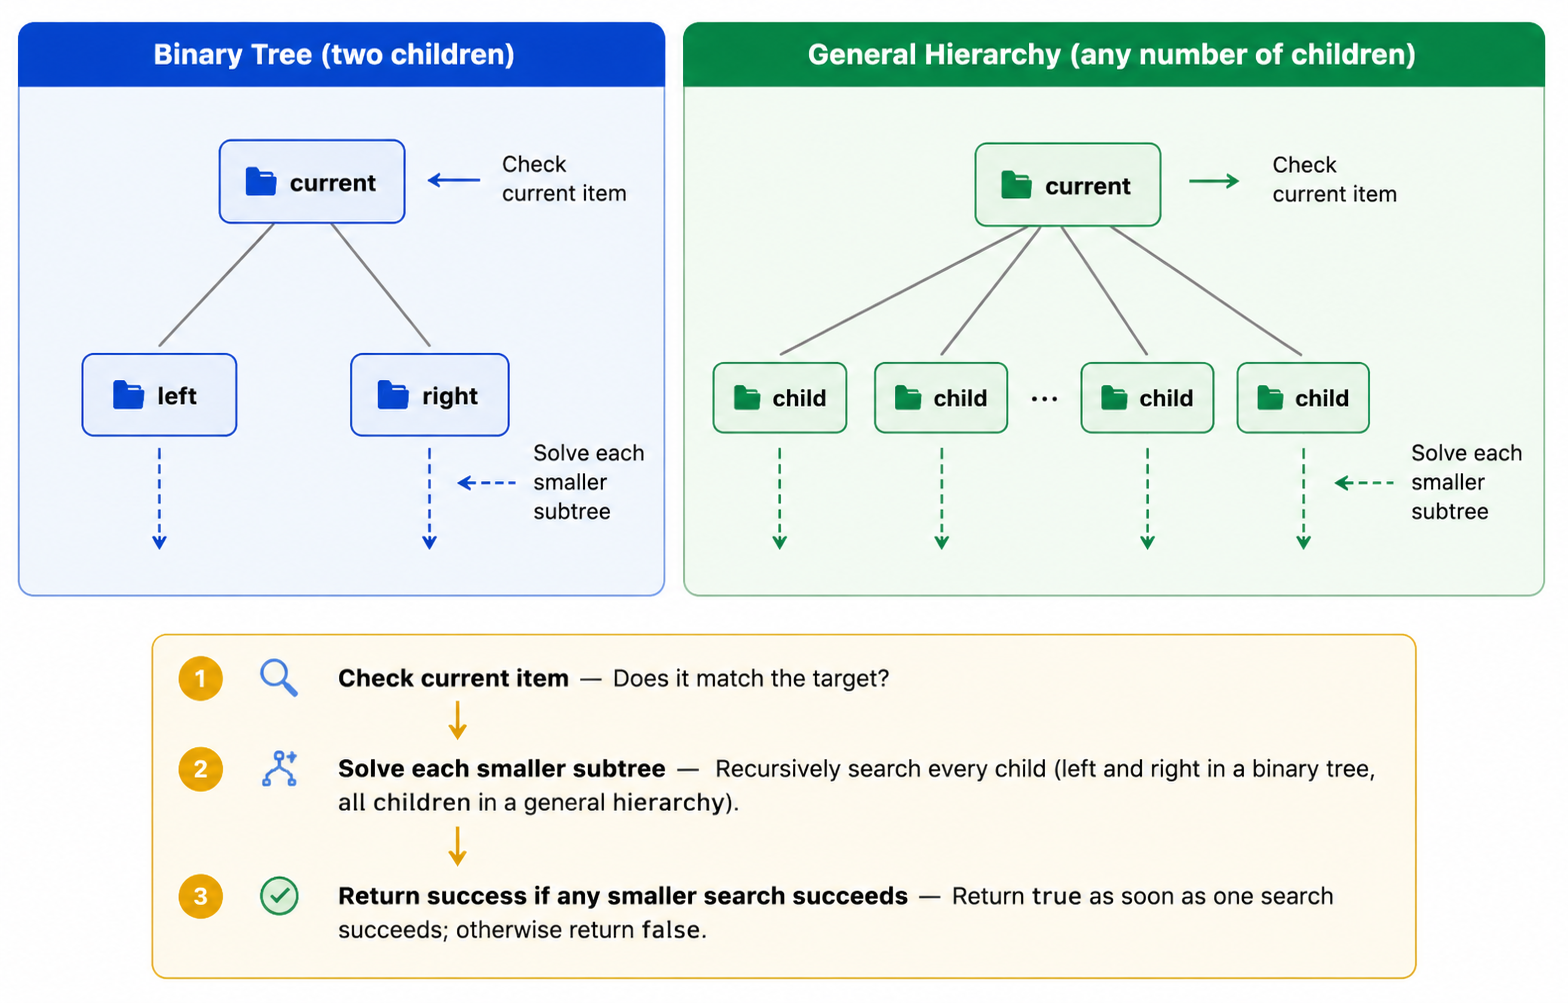
\includegraphics[width=0.9\textwidth,keepaspectratio]{../../../assets/figures/practical07/binary_vs_general}
    \caption{Comparing Binary Tree vs a more General Hierarchy.}
    \label{fig:binary_vs_general}
\end{figure}


\subsection{What Stayed the Same?}

Return to the three recursive-design questions.

\begin{center}
\begin{tabular}{p{0.34\textwidth} p{0.54\textwidth}}
\toprule
\textbf{Question} & \textbf{General Hierarchy Search} \\
\midrule
What is the smallest problem? &
An empty hierarchy or a folder with no remaining children. \\
How does the problem become smaller? &
Search one child hierarchy. \\
What work remains? &
Continue with the remaining children or return success when one search finds
the target. \\
\bottomrule
\end{tabular}
\end{center}

The representation determines how the child nodes are accessed.

The recursive idea determines that each child is solved using the same search
process.

\begin{reflectionbox}
Compare the search from Part C with the general hierarchy above.

\begin{enumerate}
    \item What part of the algorithm changed?
    \item What part remained identical?
    \item Which part belonged to the binary-tree representation?
    \item Which part belonged to recursive problem solving?
\end{enumerate}
\end{reflectionbox}

\subsection{Return to the Opening Problem}

At the start of the practical, you were asked how you would find a missing file.

You may have described a process similar to:

\begin{enumerate}
    \item inspect the current folder;
    \item stop if the target is present;
    \item otherwise search each subfolder;
    \item return whether any search succeeds.
\end{enumerate}

At the time, this was ordinary reasoning.

You can now recognise its formal structure:

\begin{itemize}
    \item the current folder is the current problem;
    \item each subfolder is a smaller version of the same problem;
    \item a folder with no remaining children provides a stopping point;
    \item Boolean results propagate back to the original search.
\end{itemize}

You had already described a recursive algorithm before the practical introduced
a binary tree.

\subsection{Final Reflection}

\begin{reflectionbox}
At the beginning of this practical, recursion may have seemed like a programming
technique.

Looking back now:

\begin{enumerate}
    \item Where was the base case in your original folder-search description?
    \item What was the smaller problem?
    \item What information did each smaller search return?
    \item Why did the binary-tree simplification help?
    \item Why was that simplification not essential?
    \item Can you identify another everyday hierarchy that could be processed
          using the same reasoning?
\end{enumerate}
\end{reflectionbox}

\subsection{Engineering Takeaway}

\begin{importantnote}
Throughout this practical, the examples changed:

\begin{center}
numerical problems
\(\rightarrow\)
folder hierarchies
\(\rightarrow\)
binary trees
\(\rightarrow\)
generic recursive algorithms
\end{center}

The recursive thinking did not change.

Experienced software engineers often recognise recurring problem structures
before they think about code. Recursion is one example of that deeper pattern
recognition.
\end{importantnote}


\section{Fast Finisher Challenges}

The following tasks are optional. Complete them only after the core tests pass
and your required work has been committed.

\begin{importantnote}
These challenges extend the recursive pattern. They are not required for
completion of the practical.
\end{importantnote}

\subsection{Challenge 1 -- Sum Every Value}

Implement a function that returns the sum of every item in an integer tree:

\begin{cppcode}
int sigma(const TreeNode<int>* tree);
\end{cppcode}

Begin with the three questions:

\begin{enumerate}
    \item What should an empty tree contribute to a sum?
    \item Which smaller trees must be summed?
    \item How should the current item and the two returned results be combined?
\end{enumerate}

A useful contract is:

\[
\operatorname{sigma}(\text{empty tree})=0
\]

and for a non-empty tree:

\[
\operatorname{sigma}(\text{tree})
=
\text{current item}
+
\operatorname{sigma}(\text{left})
+
\operatorname{sigma}(\text{right})
\]

Create your own Catch2 tests before implementing the function.

Include at least:

\begin{itemize}
    \item an empty tree;
    \item a single node;
    \item a balanced tree;
    \item negative values;
    \item an uneven tree.
\end{itemize}

\begin{reflectionbox}
Compare \mintinline{cpp}{sigma()} with \mintinline{cpp}{depth()}.

Which lines express the shared traversal?

Which lines express the different work performed at each node?
\end{reflectionbox}

\subsection{Challenge 2 -- Find the Maximum Value}

Implement:

\begin{cppcode}
int maxnum(const TreeNode<int>* tree);
\end{cppcode}

Unlike a sum, an empty tree has no natural maximum integer value.

State and document a clear precondition:

\begin{quote}
The tree passed to \mintinline{cpp}{maxnum()} must contain at least one node.
\end{quote}

Your tests should include:

\begin{itemize}
    \item a single node;
    \item the maximum at the root;
    \item the maximum in the left subtree;
    \item the maximum in the right subtree;
    \item trees containing only negative values;
    \item an uneven tree.
\end{itemize}

Be careful when one child is empty. Do not dereference a missing child merely
to obtain a comparison value.

\begin{tipbox}
This challenge is more demanding than \mintinline{cpp}{sigma()} because the
empty-tree result is not a convenient identity value.

Design the contract before writing the recursion.
\end{tipbox}

\subsection{Challenge 3 -- Count the Leaves}

Implement a generic function:

\begin{cppcode}
template <typename T>
int countLeaves(const TreeNode<T>* tree);
\end{cppcode}

A leaf is a node for which both children are empty.

Design tests for:

\begin{itemize}
    \item an empty tree;
    \item one leaf;
    \item the shared balanced file tree;
    \item a skewed tree;
    \item an uneven tree.
\end{itemize}

This challenge asks you to distinguish between:

\begin{itemize}
    \item an empty tree;
    \item a leaf;
    \item an internal node.
\end{itemize}

\subsection{Challenge 4 -- Observe Recursive Destruction}

Add temporary diagnostic output to the \mintinline{cpp}{TreeNode} destructor so
that each item is printed as it is destroyed.

Run \mintinline{text}{example02} and observe the order in which the nodes are
deleted after:

\begin{cppcode}
delete tree;
\end{cppcode}

Before running the example, predict the order.

Afterwards, remove the diagnostic output so that the supplied class returns to
its clean state.

\begin{reflectionbox}
Why are child nodes destroyed before the current node's destruction is fully
complete?

How does this compare with the return journey in the Part A demonstration?
\end{reflectionbox}


\frontsection{Wrap-up}

In this practical, you have:

\begin{itemize}
    \item designed recursion using a base case, smaller problem and waiting work;
    \item traced recursive calls and returned values;
    \item implemented a recursive Digital Root;
    \item recognised recursive structure in a folder-search problem;
    \item constructed a dynamically allocated binary tree using TDD;
    \item navigated the tree using child pointers;
    \item implemented recursive tree search;
    \item measured balanced, skewed and uneven trees;
    \item generalised a concrete search function using a template;
    \item recognised that the recursive idea extends beyond binary trees.
\end{itemize}

The most important result is not any one function.

It is the ability to ask:

\begin{enumerate}
    \item What is the smallest problem?
    \item How can the problem become smaller?
    \item What remains after the smaller problem returns?
\end{enumerate}

Those questions will reappear in later topics including divide-and-conquer
algorithms, tree traversal, graph search, parsing and algorithm analysis.

\begin{importantnote}
A recursive solution is not automatically better than an iterative one.

The engineering decision depends on whether recursion reflects the structure of
the problem clearly, whether the stopping condition is safe, and whether the
resource costs are appropriate.

In this practical, recursion was valuable because the data itself was
recursive.
\end{importantnote}


\frontsection{CSC2059 Engineering Workflow}

The work in this practical followed the CSC2059 engineering workflow.

\begin{center}
\begin{tabular}{p{0.2\textwidth} p{0.68\textwidth}}
\toprule
\textbf{Stage} & \textbf{How It Appeared in This Practical} \\
\midrule
Predict &
You predicted recursive calls, returned values and pointer-navigation output. \\
Observe &
You ran guided demonstrations and inspected targeted test failures. \\
Understand &
You connected base cases, smaller problems and waiting work to each algorithm. \\
Test &
You used focused Catch2 targets to expose one required behaviour at a time. \\
Implement &
You completed Digital Root, tree construction, search and depth. \\
Refine &
You improved incomplete solutions as deeper and uneven cases were introduced. \\
Detect Code Smell &
The integer-search test exposed that a string-only interface was unnecessarily
restrictive. \\
Refactor &
You converted the concrete search into a reusable function template while
preserving existing behaviour. \\
Reuse &
You recognised the same recursive pattern across different problems and tree
shapes. \\
\bottomrule
\end{tabular}
\end{center}

\frontsection{Submission Checklist}

Before leaving today's lab, confirm that:

\begin{itemize}
    \item The project builds successfully using \mintinline{text}{make}.
    \item All required public tests pass.
    \item The demonstration programs execute correctly.
    \item Every dynamically allocated tree is deleted correctly.
    \item No temporary debugging output remains.
    \item Your latest work has been committed and pushed to GitHub.
\end{itemize}

\begin{reflectionbox}
Before leaving the practical, complete this sentence:

\begin{quote}
I would consider recursion when a problem\ldots
\end{quote}

Your answer should describe the structure of the problem, not the syntax of a
recursive function.
\end{reflectionbox}

% End of Practical 7


\end{document}
